\section{系统分析}
\subsection{可行性分析}
\subsubsection{技术可行性分析}

本系统以 React 为整体框架,整合 three.js, ar.js 实现基于 WebGL 的 AR 交互功能。采用 fetch 技术获取后端数据以及图像识别和标记捕捉数据。整体上采用了信息系统的开发方法、网络和通信技术、数据库技术等,并且基于B/S结构规划技术和设计技术。本系统采用的绝大部分包均获得了应用级市场的认可,对于尚未广泛使用的 ar.js 包,本系统将其集成进 react 框架,成功实现了现实世界识别功能。综上,本系统开发技术是完全可行的。

\subsubsection{经济可行性分析}

本系统完全采用开源框架与技术,系统应用的支出费用主要包括系统开发费用和系统运行费用。

其中系统开发费用有:人工费用、咨询评审费用、设备费用、调研差旅费、开发软件费用以及不可预见的费用。系统运行费用主要包括:系统维护费、设备维护费、消耗材料费。

本系统带来的经济效益由以下几个方面来衡量:
\begin{enumerate}
  \item 提供预览服务: 虚拟物品与现实结合,用户对物品有更直观的视觉感受。
  \item 降低试错成本: AR 可以在虚拟环境中进行产品原型测试,减少了在实际生产环境中出现的错误和问题,节省了成本。
  \item 提高物品销售额:以为产品展示提供更加直观、生动的效果,从而吸引更多消费者购买产品。
\end{enumerate}

社会效益有:
\begin{enumerate}
  \item 提供更好的用户体验:AR 技术为校园用户提供更加直观、生动、互动的体验,从而提高用户的满意度。
  \item 促进文化创意产业的发展:交互系统可以为文化创意产业提供新的展示和推广方式,例如可以将文物、艺术品等通过 AR 技术呈现给观众,从而提高文化创意产业的影响力和发展潜力。
  \item 提高教学水平:交互系统可以为学生提供更加直观、生动的学习体验。
\end{enumerate}

\subsubsection{社会可行性分析}

基于 WebGL 的 AR 校园交互系统具有以下社会可行性:
\begin{enumerate}
  \item 促进大学校园文化建设:该系统可以通过AR技术展示大学校园的历史、文化、建筑、艺术品等方面的信息,为大学校园文化建设提供更加直观、生动的展示方式。
  \item 提高学生的学习体验:该系统可以为学生提供更加直观、生动的学习体验,例如可以将科学知识、历史文化等通过AR技术呈现给学生,从而提高学生的学习兴趣和学习效果。
  \item 提高大学校园的安全管理:该系统可以通过AR技术为学生提供安全教育,例如为学生演示火灾、地震等紧急情况的应对方法,提高学生的安全意识和应对能力,从而提高大学校园的安全管理水平。
  \item 推动 AR 技术的应用和发展: 该系统有助于激发学生对 AR 技术以及相关图像识别,三维图像显示技术的兴趣。
\end{enumerate}

\subsection{需求分析}

软件工程实践正变得越来越重要,以减轻任何可能导致代价高昂的停机时间、不正确的行为或安全故障的失败风险。需求提取是系统地从人类利益相关者、系统环境、可行性研究、市场分析、商业计划、竞争产品分析和领域知识的组合中提取和识别系统需求的过程。\cite{jabar2012software}

\subsubsection{功能性需求分析}

\begin{enumerate}
  \item 登陆注册: 
  
  用户 id 必须与学号或工作编号一致,在注册时匹配校园编号表。用户身份分为四类: 游客,学生,老师,管理员。不同的身分将获得系统的不同权限以及推送内容。
  \item 首页推送: 
  
  系统首页划分为``为你推荐'', ``最新更新'', ``我的关注''三个分区,分别获取推荐内容,最新内容以及关注内容。
  \item 3D 模型展示: 
  
  系统建立 3D 模型展示环境,获取模型数据并在手机内直接展示。且提供模型背景,预设环境等可操作选项供用户预览。同时提供一定的模型文本信息,且用户可以在简略信息与详细信息模式直接切换,也可完全屏蔽模型信息。

  \item 3D 模型 AR 预览:
  
  系统调用设备摄像头将模型放入到 AR 环境中,允许用户在现实环境中对模型进行移动缩放等操作,提供 3D 模型预览服务。

  \item AR 场景识别:
  
  根据摄像头捕捉的图像信息,采用标记捕捉或图像识别算法,在捕捉到对应信息后显示相关三维模型以及对应文本信息。
\end{enumerate}

\subsubsection{非功能性需求分析}

\begin{enumerate}
  \item 性能
  
  性能指标可分为事件性能和空间性能。
  \begin{itemize}
    \item 时间性能: 本系统操作的持续时间不超过2秒,数据连接操作的持续时间不超过5秒。系统利用浏览器异步加载机制加载需要的资源,采用非阻塞算法逐步对场景,模型加载。如果由于网络问题,数据无法获取,系统应在等待至多 10 分钟后给出提示并恢复。
    \item 空间性能: 本系统按需推送内容,在瀑布流中每次仅推送有限内容,根据用户操作增加推送内容。在 AR 场景识别过程中,根据用户地理位置推送必要数据。
  \end{itemize}

  \item 可靠性
  
  本系统测试时间不少于100小时。系统应避免因故障而引起的故障能力。在测试过程中,系统应尽可能经历所有可能出现的故障情况,以确保系统的成熟度。当硬件或软件出现异常时,系统仍应具有服务能力。业务容量减少,但不会导致系统崩溃。该系统应能在停机后十分钟内修复并正常运行。

  \item 可用性

  本系统在接收到用户输入的错误数据后,系统不会崩溃,系统能够识别错误并给用户相应的提示信息。系统界面美观,对用户具有吸引力。本系统的界面设计应在保证基本功能的基础上实现友好的布局,与市面上多数移动设备 app 界面操作保持一致。
  
  \item 易用性
  
  本系统易于学习。系统应确保操作逻辑符合常规 app 操作逻辑,新用户在第一次使用时,在3分钟的学习时间内了解整个系统的基本功能,在10分钟的学习时间内掌握系统的所有功能。AR交互系统的用户界面应该简单、直观,易于使用和导航。系统采用合适的配色、布局和图标来吸引用户的注意力,并使用户能够快速、准确地完成任务。

  \item 安全性
  
  AR交互系统具有适当的安全措施,用户的隐私和数据安全。系统应该使用HTTPS协议来保护用户的数据传输,并提供强密码、双向加密验证等安全功能。前端仅对传输来的加密数据进行验证,非必要不保留。后端对重要数据进行加密保存。

  \item 可维护性
  
  系统采用模块化设计。将系统拆分为多个独立的模块,每个模块处理特定的任务或功能。有助于提高系统的可维护性,开发人员可以更容易地定位和修复问题,并且在更新或升级时可以更轻松地进行更改。在系统设计和开发过程中,采用一致的编程规范和标准。确保代码的可读性和可维护性。使用版本控制工具(如Git)提高系统可维护性,可以协作开发和分支管理。

  \item 可扩展性
  
  系统中的各个模块应该尽可能地松耦合,以避免修改一个模块对其他模块产生意外影响。这有助于确保系统的可拓展性和稳定性。在设计和开发过程中,使用广泛采用的标准和技术,以便将来可以轻松地添加新功能或集成其他系统。
\end{enumerate}

\subsection{系统模型}

\subsubsection{用例图} 

\begin{figure}[H]
  \small
  \centering
  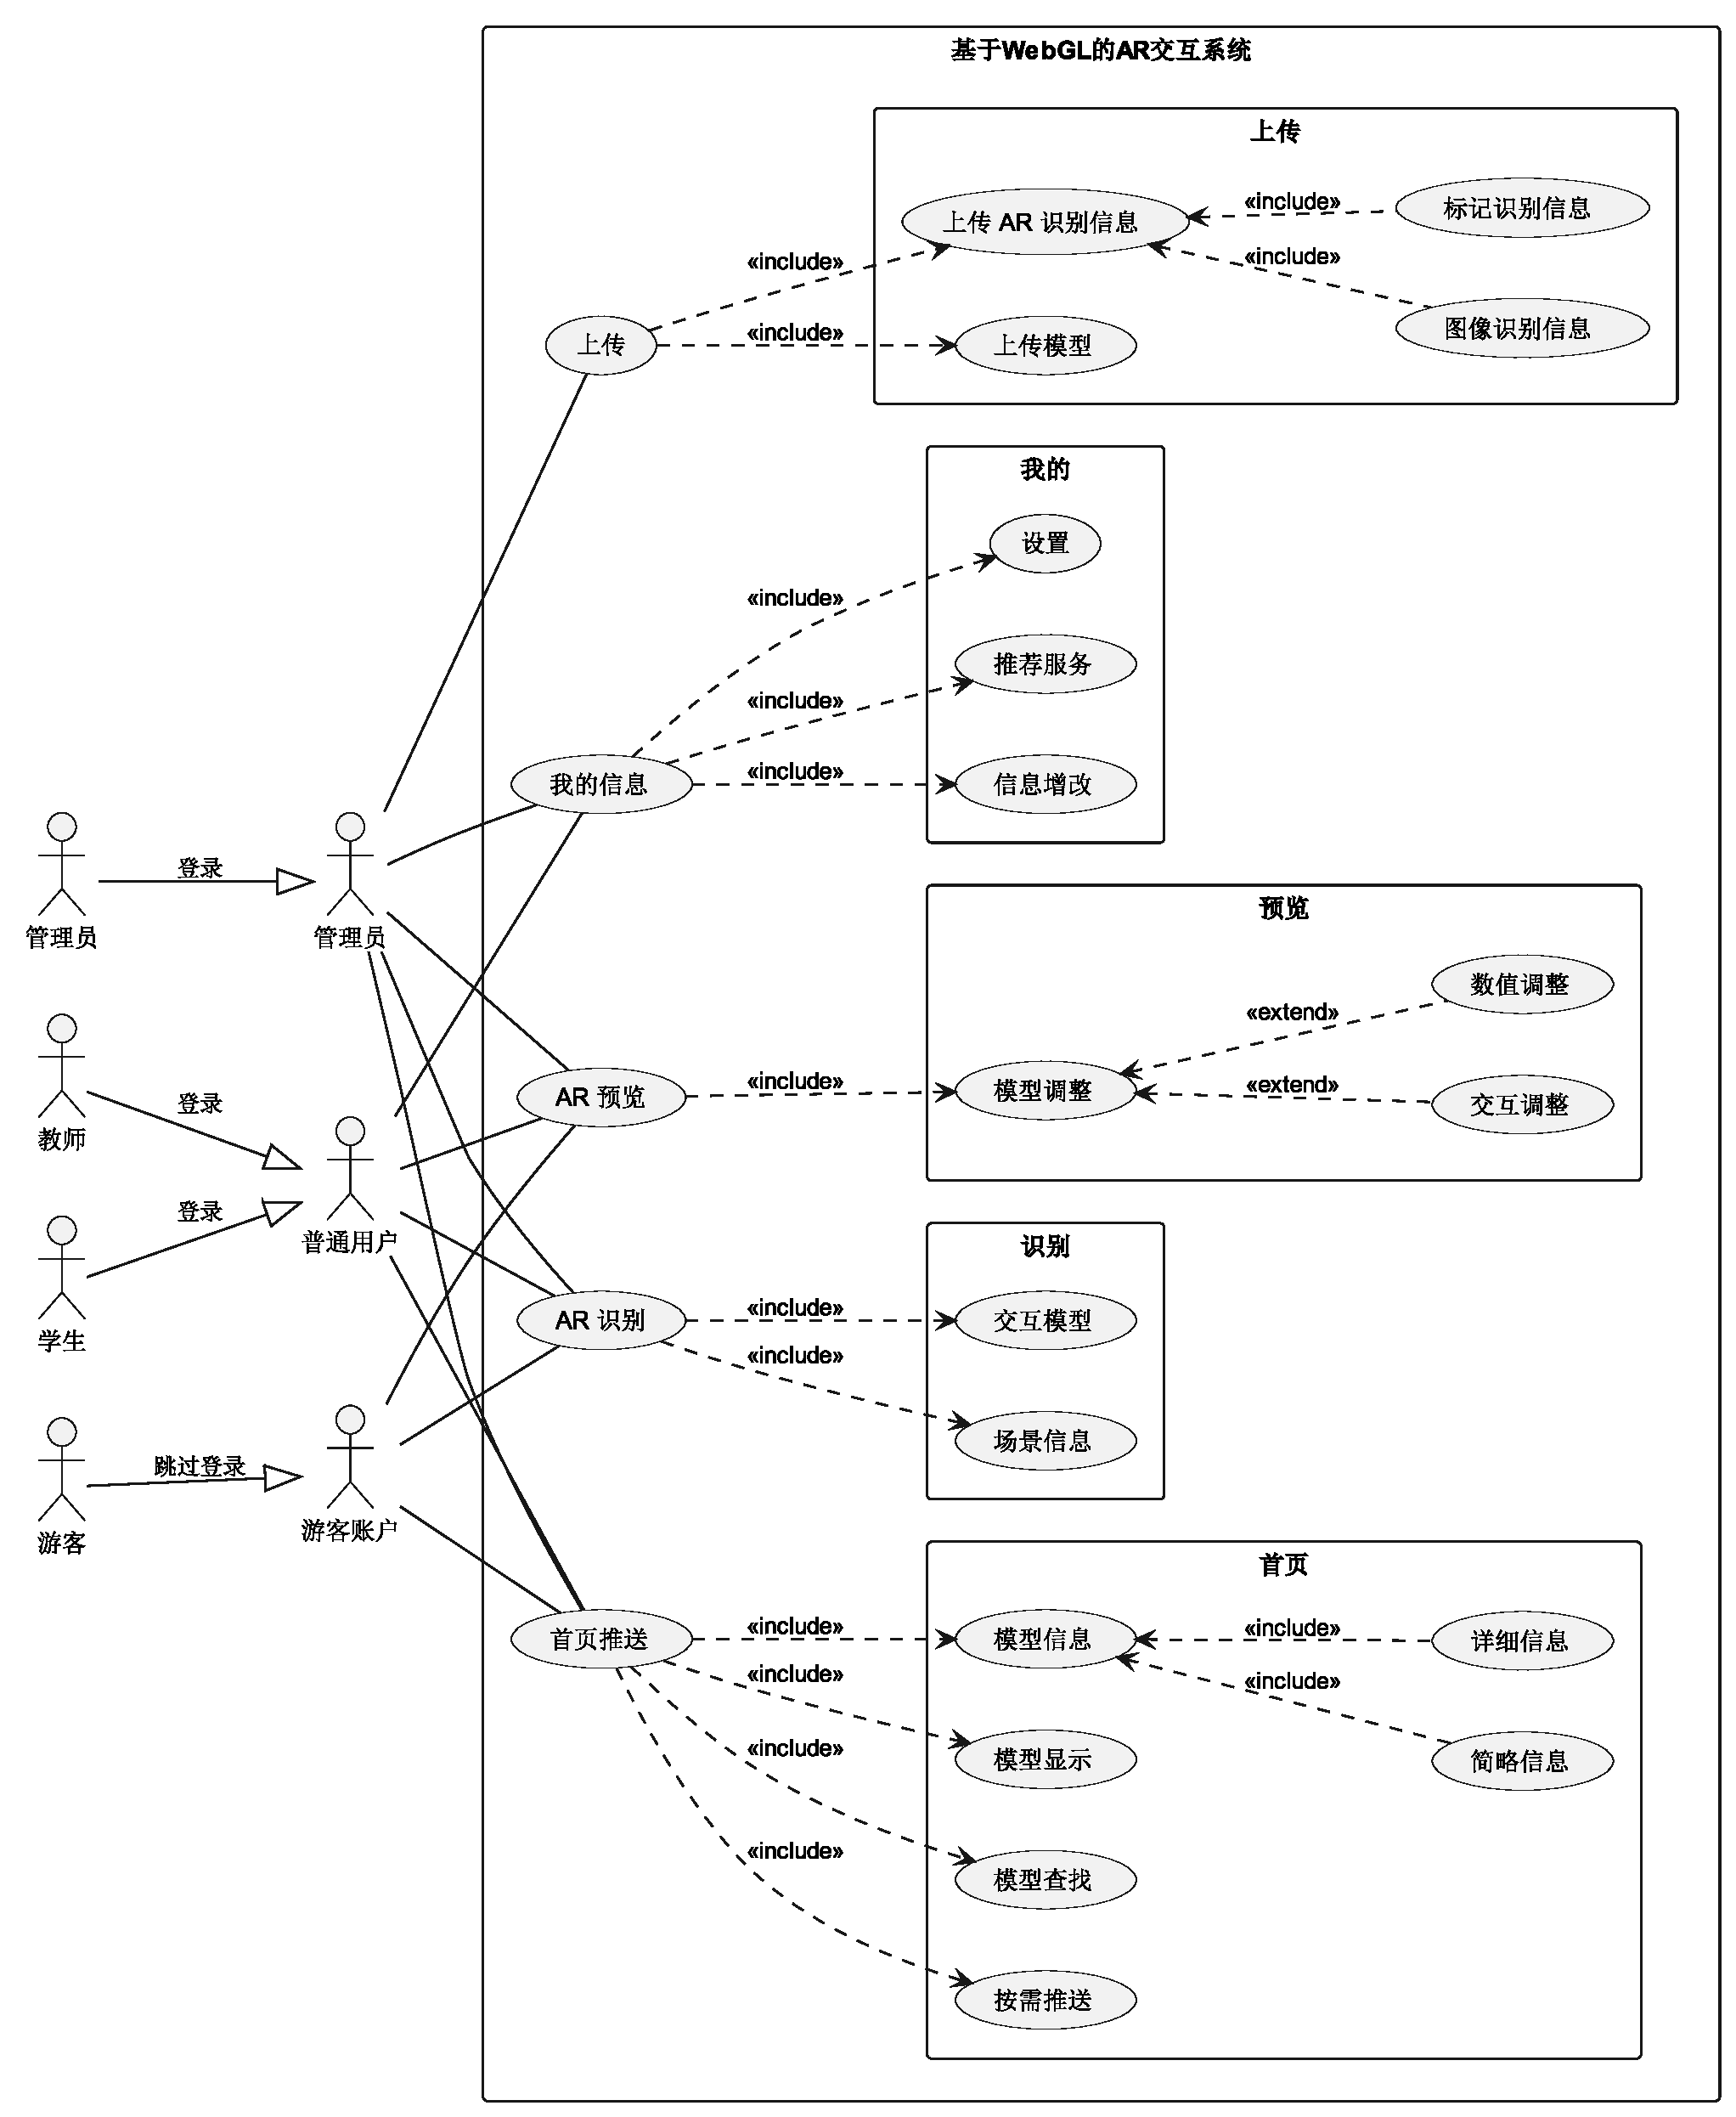
\includegraphics[width=\textwidth]{./figs/UserCase.eps}
  \caption{系统用例图}
  \label{fig:系统用例图}
\end{figure}

\subsubsection{用例表} 

\begin{table}[H]
  \centering
  \renewcommand\arraystretch{1.1}
  \small
  \caption{用户登录用例表}
  \setlength{\tabcolsep}{4mm}
  \begin{tabular}{|p{2cm}|p{5.75cm}|p{5.75cm}|}
    \hline \textbf{用例名} & \multicolumn{2}{l|}{用户登录} \\
    \hline \textbf{角色} & \multicolumn{2}{l|}{学生,职工,管理员} \\
    \hline \textbf{准入条件} & \multicolumn{2}{l|}{用户拥有进入系统的权限} \\
    \hline \textbf{事件流} & \textbf{角色步骤} & \textbf{系统步骤} \\
    \hline \multirow{3}{*}{~} & \textbf{1.} 用户进入登录界面  &    \\
    \cline{2-3} & \textbf{2.} 用户输入用户名/邮箱和密码 & \textbf{3:} 前端进行数据检查。 \\
    \cline{2-3} &  & \textbf{4:} 后端查询数据库进行匹配。 \\
    \cline{2-3} &  & \textbf{5:} 用户进入系统,跳转到``首页''界面 \\
    \hline \textbf{退出条件}  & \multicolumn{2}{l|}{系统验证用户名密码正确} \\
    \hline \multirow{2}{*}{\textbf{例外}} & \multicolumn{2}{l|}{\textbf{1.} 步骤3,前端检查数据错误,给出提示信息。} \\
     & \multicolumn{2}{l|}{\textbf{2.} 步骤4,后端匹配数据失败,用户重新登录。} \\
    \hline
  \end{tabular}
\end{table}

\begin{table}[H]
  \centering
  \renewcommand\arraystretch{1.1}
  \small
  \caption{用户注册用例表}
  \setlength{\tabcolsep}{4mm}
  \begin{tabular}{|p{2cm}|p{5.75cm}|p{5.75cm}|}
    \hline \textbf{用例名} & \multicolumn{2}{l|}{用户注册} \\
    \hline \textbf{角色} & \multicolumn{2}{l|}{学生,职工,管理员} \\
    \hline \textbf{准入条件} & \multicolumn{2}{l|}{用户拥有进入系统的权限} \\
    \hline \textbf{事件流} & \textbf{角色步骤} & \textbf{系统步骤} \\
    \hline \multirow{3}{*}{~} & \textbf{1.} 用户进入注册界面。  &    \\
    \cline{2-3} & \textbf{2.} 用户填写并提交注册信息。 & \textbf{3:} 前端进行数据检查。 \\
    \cline{2-3} &  & \textbf{4:} 后端根据校园系统表判断能否注册,并返回信息。 \\
    \cline{2-3} &  & \textbf{5:} 前端显示注册结果,跳转到``我的''界面。 \\
    \hline \textbf{退出条件}  & \multicolumn{2}{l|}{用户成功注册} \\
    \hline \multirow{2}{*}{\textbf{例外}} & \multicolumn{2}{l|}{\textbf{1.} 步骤3,前端检查数据错误,给出提示信息。} \\
     & \multicolumn{2}{l|}{\textbf{2.} 步骤4,后端未匹配到对应编号,或编号与选定的权限组不符。} \\
    \hline
  \end{tabular}
\end{table}

\begin{table}[H]
  \centering
  \renewcommand\arraystretch{1.1}
  \small
  \caption{用户增改个人信息用例表}
  \setlength{\tabcolsep}{4mm}
  \begin{tabular}{|p{2cm}|p{5.75cm}|p{5.75cm}|}
    \hline \textbf{用例名} & \multicolumn{2}{l|}{用户增改个人信息} \\
    \hline \textbf{角色} & \multicolumn{2}{l|}{学生,职工,管理员} \\
    \hline \textbf{准入条件} & \multicolumn{2}{l|}{用户拥有个人账号} \\
    \hline \textbf{事件流} & \textbf{角色步骤} & \textbf{系统步骤} \\
    \hline \multirow{3}{*}{~} & \textbf{1.} 用户进入我的界面,针对个人信息进行增改。  &    \\
    \cline{2-3} & \textbf{2.} 用户提交修改后的个人信息。 & \textbf{3:} 前端进行数据检查。 \\
    \cline{2-3} &  & \textbf{4:} 后端增改数据 \\
    \cline{2-3} &  & \textbf{5:} 前端显示增改后的结果 \\
    \hline \textbf{退出条件}  & \multicolumn{2}{l|}{成功修改信息} \\
    \hline \multirow{2}{*}{\textbf{例外}} & \multicolumn{2}{l|}{\textbf{1.} 步骤3,前端检查数据错误,给出提示信息。} \\
     & \multicolumn{2}{l|}{\textbf{2.} 步骤4,后端增改数据失败,给出错误信息。} \\
    \hline
  \end{tabular}
\end{table}

\begin{table}[H]
  \centering
  \renewcommand\arraystretch{1.1}
  \small
  \caption{用户上传模型用例表}
  \setlength{\tabcolsep}{4mm}
  \begin{tabular}{|p{2cm}|p{5.75cm}|p{5.75cm}|}
    \hline \textbf{用例名} & \multicolumn{2}{l|}{用户上传模型} \\
    \hline \textbf{角色} & \multicolumn{2}{l|}{管理员} \\
    \hline \textbf{准入条件} & \multicolumn{2}{l|}{用户拥有管理员权限} \\
    \hline \textbf{事件流} & \textbf{角色步骤} & \textbf{系统步骤} \\
    \hline \multirow{3}{*}{~} & \textbf{1.} 用户进入上传界面,选择上传模型。  &    \\
    \cline{2-3} & \textbf{2.} 用户输入模型URL,模型信息。 & \textbf{3:} 前端进行数据检查。 \\
    \cline{2-3} &  & \textbf{4:} 后端检查是否有相同数据,返回检查结果。 \\
    \cline{2-3} &  & \textbf{5:} 前端显示上传结果 \\
    \cline{2-3} & \textbf{6:} 用户确认上传结果 & \textbf{7:} 前端退出上传界面 \\
    \hline \textbf{退出条件}  & \multicolumn{2}{l|}{上传信息正确} \\
    \hline \multirow{2}{*}{\textbf{例外}} & \multicolumn{2}{l|}{\textbf{1.} 步骤3,前端检查数据错误,给出提示信息。} \\
     & \multicolumn{2}{l|}{\textbf{2.} 步骤4,后端保留数据失败,给出错误信息。} \\
    \hline
  \end{tabular}
\end{table}

\begin{table}[H]
  \centering
  \renewcommand\arraystretch{1.1}
  \small
  \caption{用户上传 AR 识别信息用例表}
  \setlength{\tabcolsep}{4mm}
  \begin{tabular}{|p{2cm}|p{5.75cm}|p{5.75cm}|}
    \hline \textbf{用例名} & \multicolumn{2}{l|}{用户上传 AR 识别信息} \\
    \hline \textbf{角色} & \multicolumn{2}{l|}{管理员} \\
    \hline \textbf{准入条件} & \multicolumn{2}{l|}{用户拥有管理员权限} \\
    \hline \textbf{事件流} & \textbf{角色步骤} & \textbf{系统步骤} \\
    \hline \multirow{3}{*}{~} & \textbf{1.} 用户进入上传界面,选择上传 AR 识别信息。  &    \\
    \cline{2-3} & \textbf{2.} 用户输入识别类型,识别图像URL,对应模型编号,相关信息。 & \textbf{3:} 前端进行数据检查。 \\
    \cline{2-3} &  & \textbf{4:} 后端检查是否有相同数据,返回检查结果。 \\
    \cline{2-3} &  & \textbf{5:} 前端显示上传结果 \\
    \cline{2-3} & \textbf{6:} 用户确认上传结果 & \textbf{7:} 前端退出上传界面 \\
    \hline \textbf{退出条件}  & \multicolumn{2}{l|}{上传信息正确} \\
    \hline \multirow{2}{*}{\textbf{例外}} & \multicolumn{2}{l|}{\textbf{1.} 步骤3,前端检查数据错误,给出提示信息。} \\
     & \multicolumn{2}{l|}{\textbf{2.} 步骤4,后端保留数据失败,给出错误信息。} \\
    \hline
  \end{tabular}
\end{table}

\begin{table}[H]
  \centering
  \renewcommand\arraystretch{1.1}
  \small
  \caption{首页推送用例表}
  \setlength{\tabcolsep}{4mm}
  \begin{tabular}{|p{2cm}|p{5.75cm}|p{5.75cm}|}
    \hline \textbf{用例名} & \multicolumn{2}{l|}{首页推送} \\
    \hline \textbf{角色} & \multicolumn{2}{l|}{游客,学生,职工,管理员} \\
    \hline \textbf{准入条件} & \multicolumn{2}{l|}{用户能够进入系统} \\
    \hline \textbf{事件流} & \textbf{角色步骤} & \textbf{系统步骤} \\
    \hline \multirow{3}{*}{~} & \textbf{1.} 用户进入首页  &    \\
    \cline{2-3} & \textbf{2.} 用户选择 ``为你推荐'',``最新更新'',``我的关注'' 任一选项 & \textbf{3:} 前端发送对应请求 \\
    \cline{2-3} &  & \textbf{4:} 后端根据请求类型与权限组查找并返回不同数据。 \\
    \cline{2-3} &  & \textbf{5:} 前端根据接受的数据类型显示模型卡。 \\
    \hline \textbf{退出条件}  & \multicolumn{2}{l|}{用户切换筛选类型} \\
    \hline \multirow{1}{*}{\textbf{例外}} & \multicolumn{2}{l|}{\textbf{1.} 步骤4,后端查询数据失败。} \\
    \hline
  \end{tabular}
\end{table}

\begin{table}[H]
  \centering
  \renewcommand\arraystretch{1.1}
  \small
  \caption{首页查询用例表}
  \setlength{\tabcolsep}{4mm}
  \begin{tabular}{|p{2cm}|p{5.75cm}|p{5.75cm}|}
    \hline \textbf{用例名} & \multicolumn{2}{l|}{首页查询} \\
    \hline \textbf{角色} & \multicolumn{2}{l|}{游客,学生,职工,管理员} \\
    \hline \textbf{准入条件} & \multicolumn{2}{l|}{用户能够进入系统} \\
    \hline \textbf{事件流} & \textbf{角色步骤} & \textbf{系统步骤} \\
    \hline \multirow{3}{*}{~} & \textbf{1.} 用户进入首页  &    \\
    \cline{2-3} & \textbf{2.} 用户进行关键字搜索 & \textbf{3:} 前端检查搜索内容并发送对应请求 \\
    \cline{2-3} &  & \textbf{4:} 后端根据请求与权限组查找数据并返回。 \\
    \cline{2-3} &  & \textbf{5:} 前端根据接受的数据类型显示模型卡。 \\
    \hline \textbf{退出条件}  & \multicolumn{2}{l|}{用户点击``搜索''按钮} \\
    \hline \multirow{2}{*}{\textbf{例外}} & \multicolumn{2}{l|}{\textbf{1.} 步骤3,搜索内容出错。} \\
     & \multicolumn{2}{l|}{\textbf{2.} 步骤4,后端查询数据失败。} \\
    \hline
  \end{tabular}
\end{table}

\begin{table}[H]
  \centering
  \renewcommand\arraystretch{1.1}
  \small
  \caption{模型展示用例表}
  \setlength{\tabcolsep}{4mm}
  \begin{tabular}{|p{2cm}|p{5.75cm}|p{5.75cm}|}
    \hline \textbf{用例名} & \multicolumn{2}{l|}{模型展示} \\
    \hline \textbf{角色} & \multicolumn{2}{l|}{游客,学生,职工,管理员} \\
    \hline \textbf{准入条件} & \multicolumn{2}{l|}{用户能够进入系统} \\
    \hline \textbf{事件流} & \textbf{角色步骤} & \textbf{系统步骤} \\
    \hline \multirow{3}{*}{~} & \textbf{1.} 用户进入首页  &    \\
    \cline{2-3} & \textbf{2.} 用户点击对应模型卡。 & \textbf{3:} 前端向后端请求模型详细信息数据。 \\
    \cline{2-3} &  & \textbf{4:} 后端返回模型数据。 \\
    \cline{2-3} &  & \textbf{5:} 前端加载界面与模型。 \\
    \cline{2-3} & \textbf{6:} 用户点击交互按钮。 & \textbf{7:} 前端做出对应响应。 \\
    \cline{2-3} & \textbf{8:} 用户退出``模型展示''界面 &  \\
    \hline \textbf{退出条件}  & \multicolumn{2}{l|}{用户退出``模型展示''界面} \\
    \hline \multirow{1}{*}{\textbf{例外}} & \multicolumn{2}{l|}{\textbf{1.} 步骤5,网络等问题加载模型或信息失败。} \\
    \hline
  \end{tabular}
\end{table}

\begin{table}[H]
  \centering
  \renewcommand\arraystretch{1.1}
  \small
  \caption{AR 预览用例表}
  \setlength{\tabcolsep}{4mm}
  \begin{tabular}{|p{2cm}|p{5.75cm}|p{5.75cm}|}
    \hline \textbf{用例名} & \multicolumn{2}{l|}{AR 预览} \\
    \hline \textbf{角色} & \multicolumn{2}{l|}{游客,学生,职工,管理员} \\
    \hline \textbf{准入条件} & \multicolumn{2}{l|}{用户能够进入系统} \\
    \hline \textbf{事件流} & \textbf{角色步骤} & \textbf{系统步骤} \\
    \hline \multirow{3}{*}{~} & \textbf{1.} 用户进入``首页''界面。  &    \\
    \cline{2-3} & \textbf{2.} 用户点击模型卡并选择 AR 预览功能。 & \textbf{3:} 跳转至``预览''界面。 \\
    \cline{2-3} &  & \textbf{4:} 系统请求设备开启摄像头与 AR 服务。 \\
    \cline{2-3} &  & \textbf{5:} 向后端请求模型数据。 \\
    \cline{2-3} &  & \textbf{6:} 前端加载模型,展示 AR 预览界面。 \\
    \cline{2-3} & \textbf{7:} 用户操作 AR 预览界面 & \textbf{8:} 前端做出对应响应。 \\
    \cline{2-3} & \textbf{9:} 用户退出``AR 模型展示''界面。 &  \\
    \hline \textbf{退出条件}  & \multicolumn{2}{l|}{用户退出``AR 模型展示''界面。} \\
    \hline \multirow{2}{*}{\textbf{例外}} & \multicolumn{2}{l|}{\textbf{1.} 步骤4,系统请求摄像头权限或 AR 服务被拒。} \\
    & \multicolumn{2}{l|}{\textbf{2.} 步骤6,网络等问题加载模型或信息失败。} \\
    \hline
  \end{tabular}
\end{table}

\begin{table}[H]
  \centering
  \renewcommand\arraystretch{1.1}
  \small
  \caption{AR 识别用例表}
  \setlength{\tabcolsep}{4mm}
  \begin{tabular}{|p{2cm}|p{5.75cm}|p{5.75cm}|}
    \hline \textbf{用例名} & \multicolumn{2}{l|}{AR 识别} \\
    \hline \textbf{角色} & \multicolumn{2}{l|}{游客,学生,职工,管理员} \\
    \hline \textbf{准入条件} & \multicolumn{2}{l|}{用户能够进入系统} \\
    \hline \textbf{事件流} & \textbf{角色步骤} & \textbf{系统步骤} \\
    \hline \multirow{3}{*}{~} & \textbf{1.} 用户进入``识别''界面  & \textbf{2:} 系统请求设备开启摄像头与 AR 服务   \\
    \cline{2-3} &  & \textbf{3:} 系统根据地理位置按需加载识别信息。\\
    \cline{2-3} &  & \textbf{4:} 系统通过图像识别或标记捕捉算法实时匹配摄像头传输的场景信息。 \\
    \cline{2-3} &  & \textbf{5:} 捕捉到有效信息。显示模型或相关提示。 \\
    \cline{2-3} & \textbf{6:} 用户与系统交互 & \textbf{7:} 系统做出响应。 \\
    \cline{2-3} & \textbf{8:} 用户退出``AR 识别'界面  &  \\
    \hline \textbf{退出条件}  & \multicolumn{2}{l|}{用户退出``AR 识别''界面} \\
    \hline \multirow{2}{*}{\textbf{例外}} & \multicolumn{2}{l|}{\textbf{1.} 步骤2,系统请求摄像头权限或 AR 服务被拒。} \\
    & \multicolumn{2}{l|}{\textbf{2.} 步骤3,网络等问题加载模型或信息失败。} \\
    \hline
  \end{tabular}
\end{table}

(3) 类图